\documentclass[conference]{IEEEtran}

% --- Packages ---
\usepackage{cite}
\usepackage{amsmath,amssymb,amsfonts}
\usepackage{algorithmic}
\usepackage{graphicx}
\usepackage{textcomp}
\usepackage{xcolor}
\usepackage{booktabs}
\usepackage{multirow}
\usepackage{array}
\usepackage{tabularx}
\usepackage{url}
\usepackage{microtype}
\usepackage{tikz}
\usetikzlibrary{shapes.geometric, arrows.meta, positioning, fit, calc, backgrounds}

% --- Micro-spacing parameters for exact 4-page fit ---
\setlength{\textfloatsep}{6pt plus 2pt minus 2pt}
\setlength{\intextsep}{6pt plus 2pt minus 2pt}
\setlength{\floatsep}{6pt plus 2pt minus 2pt}
\setlength{\dbltextfloatsep}{6pt plus 2pt minus 2pt}
\setlength{\dblfloatsep}{6pt plus 2pt minus 2pt}

\begin{document}

% --- Title & Authors ---
\title{TokenShield: A Domain-Agnostic, Real-Time Multi-Signal Behavioral Engine for Session Hijacking Detection and Automated Mitigation}

\author{
\IEEEauthorblockN{Aman Kshirsagar, Vedant Dhamele, Yash Shashank Pachhade, Yash Nandanwar}
\IEEEauthorblockA{\textit{Department of Artificial Intelligence and Data Science} \\
\textit{Yeshwantrao Chavan College of Engineering}, Nagpur, Maharashtra, India}
}

\maketitle

% --- Abstract ---
\begin{abstract}
Session hijacking, in which an adversary steals or replays a valid authentication token to impersonate a legitimate user, threatens any system that relies on bearer-token authentication after login. Because a hijacked token is, by construction, a syntactically valid credential, static web application firewalls and fixed-rate IP throttling are structurally blind to it. This paper presents TokenShield, a framework-agnostic middleware security engine that continuously evaluates every authenticated request against a seven-signal behavioral risk model spanning IP reputation, request velocity, session consistency, payload inspection, behavioral biometrics, geographic plausibility, and endpoint sensitivity. When the aggregated anomaly score crosses a calibrated critical threshold, TokenShield autonomously executes an eight-stage progressive mitigation pipeline that revokes the compromised token at the cache layer, propagates the block to the reverse-proxy edge, bans the offending device fingerprint, escalates account-level authentication, and notifies both the affected user and system administrators, without human intervention. We present the system architecture and packet-level request-mitigation flow, the mathematical formulation of the anomaly-scoring function, a comparative literature review, and an ethically-sourced, non-synthetic data-collection methodology combining genuine multi-user traffic, self-executed red-team exploitation, and public intrusion-detection benchmark corpora. We further describe the unsupervised training procedure, evaluation protocol, and a productization roadmap that generalizes the system from a banking-application demonstrator into deployable, domain-agnostic security middleware for any session-authenticated software stack.
\end{abstract}

\begin{IEEEkeywords}
session hijacking, token theft, anomaly detection, isolation forest, behavioral biometrics, intrusion detection, JSON Web Token, Redis, real-time mitigation, framework-agnostic middleware
\end{IEEEkeywords}

% ==============================================================================
\section{Introduction}
% ==============================================================================
The near-universal adoption of stateless, token-based authentication -- most commonly JSON Web Tokens (JWTs) -- has simplified horizontal scaling of web services but has concentrated an application's entire trust boundary into a single bearer credential~\cite{jones2015jwt}. Once an attacker obtains a valid token, whether through cross-site scripting, man-in-the-middle interception, malicious browser extensions, or network sniffing, the system has no cryptographic means of distinguishing the legitimate owner from the impersonator, since the token remains structurally valid until its stated expiry~\cite{owasp2021top10}. This threat is not confined to a single vertical: a hijacked session can authorize a monetary transfer in a banking app, exfiltrate patient records in a healthcare portal, or grant administrative control in an internal SaaS console within seconds of compromise.

Existing defensive layers are largely insufficient. Static web application firewalls filter on known malicious signatures and are blind to a syntactically valid, stolen token. Fixed-window IP rate limiting is evaded by low-and-slow attacks or residential proxy pools. Multi-factor authentication is effective at the login boundary but typically does not re-verify identity for the remaining lifetime of an already-issued session.

This paper introduces TokenShield, a continuous, request-level risk-evaluation engine that treats every authenticated HTTP request as a fresh trust decision rather than a one-time login event. TokenShield was implemented and validated against NeoVault, a representative digital banking application, but its detection middleware, session model, and mitigation pipeline make no banking-specific assumption: every signal it consumes -- IP, User-Agent, endpoint sensitivity, payload, geo-velocity, device fingerprint, and client telemetry -- is present in essentially any authenticated web, mobile-backend, or enterprise system. The contributions of this paper are:
\begin{itemize}
    \item A seven-signal, weighted behavioral risk-scoring formulation that fuses network-, session-, payload-, and geography-level evidence into a single bounded anomaly score computable within the request-handling critical path.
    \item A comparative literature review positioning TokenShield's fused, request-level scoring against prior single-signal anomaly-detection, fingerprinting, and biometric work.
    \item An eight-stage, fully automated mitigation pipeline spanning cache-layer token revocation, edge-proxy IP blocking, device-fingerprint banning, and account-level authentication escalation, together with a packet-level view of how a single malicious request traverses and triggers this pipeline end-to-end.
    \item An ethically-sourced, non-synthetic data-collection methodology combining genuine multi-user production traffic, controlled self-executed red-team exploitation from geographically distributed infrastructure, and established public intrusion-detection benchmark corpora.
    \item A productization roadmap converting the system from an integrated banking demonstrator into a framework-agnostic, API-based security middleware deployable in front of any session-authenticated application.
\end{itemize}

% ==============================================================================
\section{Related Work}
% ==============================================================================
Anomaly-based intrusion detection rests on the observation that attack traffic occupies sparse, separable regions of a well-chosen feature space. Liu et al.\ formalized this through the Isolation Forest algorithm, which isolates anomalies via random recursive partitioning rather than modeling a dense normal-behavior profile, yielding linear time complexity suited to streaming, low-latency deployment~\cite{liu2008isolation}. Sharafaldin et al.\ introduced CIC-IDS2018, a labeled corpus combining benign background traffic with brute-force, denial-of-service, web-attack, and infiltration classes~\cite{sharafaldin2018ids2018}. Moustafa and Slay proposed UNSW-NB15, generated on the IXIA PerfectStorm testbed to combine real background activity with nine synthesized attack categories~\cite{moustafa2015unsw}. Freeman et al.\ modeled login authenticity probabilistically from IP, device, and velocity features~\cite{freeman2016whoareyou}. Eckersley quantified how much entropy a browser's configuration alone reveals about device identity~\cite{eckersley2010unique}, while Nikiforakis et al.\ catalogued the broader web-fingerprinting ecosystem~\cite{nikiforakis2013cookieless}. Killourhy and Maxion benchmarked keystroke-dynamics classifiers as a behavioral-biometric anomaly channel~\cite{killourhy2009keystroke}. Furthermore, OWASP lists broken authentication and session management among its top web-application risks~\cite{owasp2021top10}.

Table~\ref{tab:related_work} summarizes these works against TokenShield. The common thread is that each prior contribution advances exactly one signal family, and none couples detection directly to an automated, multi-layer response. TokenShield's contribution is architectural: it fuses seven previously siloed signal families into one bounded, per-request score and wires that score directly into a cache-, edge-, device-, and account-layer mitigation pipeline, rather than treating detection and response as separate concerns.

% --- TABLE I: RELATED WORK ---
\begin{table}[!htbp]
\caption{Comparative Literature Review}
\label{tab:related_work}
\centering
\scriptsize
\renewcommand{\arraystretch}{1.3}
\begin{tabularx}{\linewidth}{>{\raggedright\arraybackslash}p{1.85cm} >{\raggedright\arraybackslash}X >{\raggedright\arraybackslash}X >{\raggedright\arraybackslash}X}
\toprule
\textbf{Ref. \& Work} & \textbf{Major Contribution} & \textbf{Limitation} & \textbf{Relation to TokenShield} \\
\midrule
\cite{liu2008isolation} Liu (2008) & Linear-time anomaly isolation via partitioning & Generic; not coupled to request feature set & Forms unsupervised ML model \\
\cite{freeman2016whoareyou} Freeman (2016) & Probabilistic takeover detection at login & Evaluated only at login, not session lifetime & Extends signal family to every request \\
\cite{sharafaldin2018ids2018} CIC-IDS (2018) & Relabeled benign/attack flow corpus & Network-flow granularity; no session semantics & External validation benchmark corpus \\
\cite{moustafa2015unsw} UNSW-NB (2015) & Hybrid real/synthetic multi-class attack data & Synthesized attack classes & External validation benchmark corpus \\
\cite{eckersley2010unique} Eckersley (2010) & Entropy quantification of device configs & Identifies devices; no real-time response & Motivates device-fingerprint signal/ban \\
\cite{nikiforakis2013cookieless} Nikiforakis (2013) & Survey of industrial fingerprinting & Descriptive survey; no scoring pipeline & Informs client telemetry design \\
\cite{killourhy2009keystroke} Killourhy (2009) & Benchmarked typing-cadence classifiers & Single modality; no network/geo fusion & Generalized into biometric signal \\
\bottomrule
\end{tabularx}
\end{table}

% ==============================================================================
\section{System Architecture}
% ==============================================================================
TokenShield is deployed as a fully containerized system with strict service-level network isolation (Fig.~\ref{fig:arch}). Client traffic first reaches an Nginx reverse proxy, which enforces edge-level rate-limiting zones and dynamically reloads a blocklist file populated by the detection engine; a lightweight watcher process polls this file's checksum and issues \texttt{nginx -s reload} within five seconds of any change. Requests are then forwarded to the Flask application server, which hosts the detection middleware, the host application's business logic, and its REST blueprints behind a single \texttt{before\_request} hook -- guaranteeing that no downstream route, however recently added, can execute before passing the risk-scoring stage. The detection engine consults a Redis in-memory store for constant-time lookups of token blocklists (\texttt{ts:block:*}), IP velocity counters (\texttt{ts:vel:*}), device-fingerprint bans (\texttt{ts:fp:*}), and geo-session history (\texttt{ts:geo:*}), with an in-process fallback if Redis becomes unreachable, while durable state -- accounts, sessions, behavior logs, and incident records -- is persisted via SQLAlchemy to a relational store. Authorized load-test and vulnerability-scanning traffic, and, during evaluation, red-team exploitation traffic, are routed directly to the application server so as to exercise the detection engine under controlled conditions without edge-level interference, a path kept logically distinct from the reverse-proxy path.

% --- FIGURE 1: ARCHITECTURE DIAGRAM ---
\begin{figure}[!htbp]
\centering
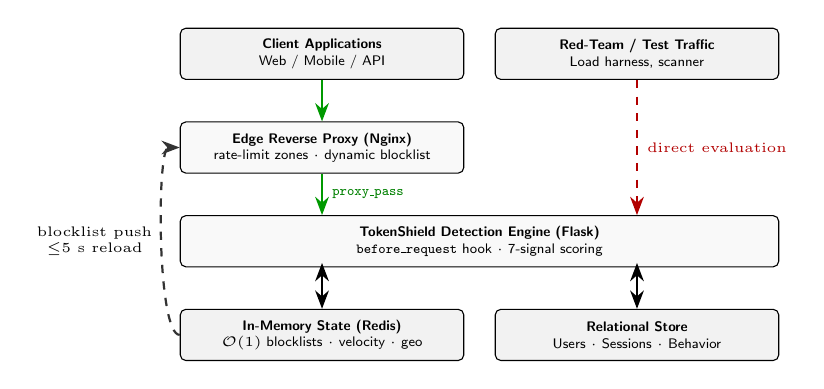
\begin{tikzpicture}[x=1.0cm, y=0.85cm, >=Stealth, font=\sffamily\tiny]
  % Top Row: Client Applications (Left) & Red-Team / Test Traffic (Right)
  \node[draw=black, fill=gray!10, rounded corners=2pt, minimum width=3.6cm, minimum height=0.65cm, align=center] (clients) at (-2.0,0) {\textbf{Client Applications}\\Web / Mobile / API};
  \node[draw=black, fill=gray!10, rounded corners=2pt, minimum width=3.6cm, minimum height=0.65cm, align=center] (redteam) at (2.0,0) {\textbf{Red-Team / Test Traffic}\\Load harness, scanner};

  % Middle Row 1: Edge Reverse Proxy (Nginx) under Client Apps
  \node[draw=black, fill=gray!5, rounded corners=2pt, minimum width=3.6cm, minimum height=0.65cm, align=center] (proxy) at (-2.0,-1.4) {\textbf{Edge Reverse Proxy (Nginx)}\\rate-limit zones $\cdot$ dynamic blocklist};

  % Middle Row 2: Detection Engine (Spans across middle)
  \node[draw=black, fill=gray!5, rounded corners=2pt, minimum width=7.6cm, minimum height=0.65cm, align=center] (engine) at (0,-2.8) {\textbf{TokenShield Detection Engine (Flask)}\\\texttt{before\_request} hook $\cdot$ 7-signal scoring};

  % Bottom Row: Redis (Left) & Database (Right)
  \node[draw=black, fill=gray!10, rounded corners=2pt, minimum width=3.6cm, minimum height=0.65cm, align=center] (redis) at (-2.0,-4.2) {\textbf{In-Memory State (Redis)}\\$\mathcal{O}(1)$ blocklists $\cdot$ velocity $\cdot$ geo};
  \node[draw=black, fill=gray!10, rounded corners=2pt, minimum width=3.6cm, minimum height=0.65cm, align=center] (db) at (2.0,-4.2) {\textbf{Relational Store}\\Users $\cdot$ Sessions $\cdot$ Behavior};

  % Connections
  % Client -> Proxy
  \draw[->, thick, draw=green!60!black] (clients) -- (proxy);

  % Proxy -> Engine (left side at x=-2.0)
  \draw[->, thick, draw=green!60!black] (proxy) -- node[right, font=\tiny, text=green!50!black] {\texttt{proxy\_pass}} (proxy |- engine.north);

  % Red-Team -> Engine (right side at x=2.0, direct bypass, no intersection with proxy!)
  \draw[->, thick, dashed, draw=red!70!black] (redteam) -- node[right, font=\tiny, text=red!70!black] {direct evaluation} (redteam |- engine.north);

  % Engine <-> Redis & DB
  \draw[<->, thick] (-2.0,-3.125) -- (redis.north);
  \draw[<->, thick] (2.0,-3.125) -- (db.north);

  % Blocklist Push Curve from Redis to Proxy (drawn cleanly on the left side)
  \draw[->, thick, dashed, draw=black!80] (redis.west) .. controls (-4.1,-4.2) and (-4.1,-1.4) .. node[left, align=center, font=\tiny] {blocklist push\\$\le$5~s reload} (proxy.west);

\end{tikzpicture}
\caption{TokenShield container-level system architecture.}
\label{fig:arch}
\end{figure}

% ==============================================================================
\section{Threat Detection Methodology}
% ==============================================================================
\subsection{Seven-Signal Anomaly Scoring}
For every authenticated request, TokenShield computes seven independent, weighted risk signals $s_1, \dots, s_7$, each bounded by an empirically calibrated weight cap, and aggregates them into a single anomaly score $S \in [0, 1]$:
\begin{equation}
S = \min\left( \sum_{i=1}^{7} s_i, ~ 1.0 \right)
\label{eq:score}
\end{equation}

Table~\ref{tab:signals} summarizes each signal, its weight cap, and its detection mechanism. The geographic-impossibility signal $s_6$ is computed from consecutive request coordinates $(\varphi_1, \lambda_1)$ and $(\varphi_2, \lambda_2)$ using the Haversine great-circle distance:
\begin{equation}
d = 2r \arcsin \left( \sqrt{\sin^2 \frac{\Delta \varphi}{2} + \cos \varphi_1 \cos \varphi_2 \sin^2 \frac{\Delta \lambda}{2}} \right)
\label{eq:haversine}
\end{equation}
where $r$ is the Earth's mean radius. The implied velocity $v = d/\Delta t$ is compared against a commercial-aviation ceiling of $900\,\text{km/h}$; any request implying a physically implausible relocation contributes to $s_6$.

% --- TABLE II: SIGNALS ---
\begin{table}[!htbp]
\caption{Seven-Signal Behavioral Risk Model}
\label{tab:signals}
\centering
\scriptsize
\renewcommand{\arraystretch}{1.25}
\begin{tabularx}{\linewidth}{c >{\raggedright\arraybackslash}p{2.2cm} c >{\raggedright\arraybackslash}X}
\toprule
\textbf{\#} & \textbf{Signal} & \textbf{Cap} & \textbf{Mechanism} \\
\midrule
1 & IP Reputation & 0.25 & Tor/botnet/datacenter CIDR match \\
2 & Request Velocity & 0.30 & Redis sliding-window INCR over 60~s \\
3 & Session Consistency & 0.30 & IP (+0.20), UA (+0.10) drift vs. origin \\
4 & Payload Analysis & 0.40 & Regex inspection for SQLi/XSS \\
5 & Behavioral Biometrics & 0.25 & Client mouse velocity, typing cadence \\
6 & Geo-Impossibility & 0.35 & Haversine distance velocity $>900\,\text{km/h}$ \\
7 & Endpoint Risk & 0.20 & Static uplift for sensitive routes \\
\bottomrule
\end{tabularx}
\end{table}

\subsection{Threat Level Classification}
The aggregated score $S$ is mapped to a discrete threat level used for both dashboard reporting and mitigation triggering:
\begin{equation}
\text{Threat}(S) = 
\begin{cases} 
\text{Critical,} & S \ge 0.85 \\
\text{High,} & 0.70 \le S < 0.85 \\
\text{Medium,} & 0.50 \le S < 0.70 \\
\text{Low,} & 0.30 \le S < 0.50 \\
\text{Safe,} & S < 0.30 
\end{cases}
\label{eq:threat}
\end{equation}
Only the Critical tier autonomously triggers the mitigation pipeline of Section~\ref{sec:mitigation}; lower tiers are logged for retrospective analysis and future retraining.

% ==============================================================================
\section{Automated Mitigation Pipeline}
\label{sec:mitigation}
% ==============================================================================
Upon reaching the critical threshold, TokenShield executes an eight-stage mitigation sequence in a background thread so as not to block the originating request's response latency, instrumented with per-stage latency measurements (Fig.~\ref{fig:mitigation}). The design deliberately layers defenses at four trust boundaries: the token layer via Redis revocation, the network edge via Nginx, the device layer via fingerprint banning -- which prevents an attacker from simply re-authenticating on the same physical device -- and the account layer via forced two-factor step-up, which protects against the possibility that the underlying credential, not merely the session token, is compromised.

% --- FIGURE 2: MITIGATION PIPELINE ---
\begin{figure}[!htbp]
\centering
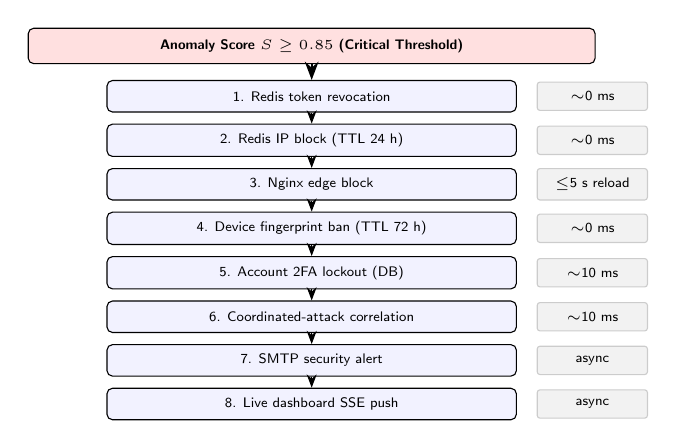
\begin{tikzpicture}[node distance=0.18cm, >=Stealth, font=\sffamily\tiny]
  \node[draw=black, fill=red!12, rounded corners=2pt, minimum width=7.2cm, minimum height=0.45cm, align=center, font=\bfseries\sffamily\tiny] (top) {Anomaly Score $S \ge 0.85$ (Critical Threshold)};

  \node[draw=black, fill=blue!5, rounded corners=2pt, minimum width=5.2cm, minimum height=0.4cm, align=center, below=0.20cm of top] (s1) {1. Redis token revocation};
  \node[draw=gray!40, fill=gray!10, rounded corners=1pt, minimum width=1.4cm, minimum height=0.36cm, align=center, font=\tiny\sffamily, right=0.25cm of s1] (t1) {$\sim$0~ms};

  \node[draw=black, fill=blue!5, rounded corners=2pt, minimum width=5.2cm, minimum height=0.4cm, align=center, below=0.14cm of s1] (s2) {2. Redis IP block (TTL 24~h)};
  \node[draw=gray!40, fill=gray!10, rounded corners=1pt, minimum width=1.4cm, minimum height=0.36cm, align=center, font=\tiny\sffamily, right=0.25cm of s2] (t2) {$\sim$0~ms};

  \node[draw=black, fill=blue!5, rounded corners=2pt, minimum width=5.2cm, minimum height=0.4cm, align=center, below=0.14cm of s2] (s3) {3. Nginx edge block};
  \node[draw=gray!40, fill=gray!10, rounded corners=1pt, minimum width=1.4cm, minimum height=0.36cm, align=center, font=\tiny\sffamily, right=0.25cm of s3] (t3) {$\le$5~s reload};

  \node[draw=black, fill=blue!5, rounded corners=2pt, minimum width=5.2cm, minimum height=0.4cm, align=center, below=0.14cm of s3] (s4) {4. Device fingerprint ban (TTL 72~h)};
  \node[draw=gray!40, fill=gray!10, rounded corners=1pt, minimum width=1.4cm, minimum height=0.36cm, align=center, font=\tiny\sffamily, right=0.25cm of s4] (t4) {$\sim$0~ms};

  \node[draw=black, fill=blue!5, rounded corners=2pt, minimum width=5.2cm, minimum height=0.4cm, align=center, below=0.14cm of s4] (s5) {5. Account 2FA lockout (DB)};
  \node[draw=gray!40, fill=gray!10, rounded corners=1pt, minimum width=1.4cm, minimum height=0.36cm, align=center, font=\tiny\sffamily, right=0.25cm of s5] (t5) {$\sim$10~ms};

  \node[draw=black, fill=blue!5, rounded corners=2pt, minimum width=5.2cm, minimum height=0.4cm, align=center, below=0.14cm of s5] (s6) {6. Coordinated-attack correlation};
  \node[draw=gray!40, fill=gray!10, rounded corners=1pt, minimum width=1.4cm, minimum height=0.36cm, align=center, font=\tiny\sffamily, right=0.25cm of s6] (t6) {$\sim$10~ms};

  \node[draw=black, fill=blue!5, rounded corners=2pt, minimum width=5.2cm, minimum height=0.4cm, align=center, below=0.14cm of s6] (s7) {7. SMTP security alert};
  \node[draw=gray!40, fill=gray!10, rounded corners=1pt, minimum width=1.4cm, minimum height=0.36cm, align=center, font=\tiny\sffamily, right=0.25cm of s7] (t7) {async};

  \node[draw=black, fill=blue!5, rounded corners=2pt, minimum width=5.2cm, minimum height=0.4cm, align=center, below=0.14cm of s7] (s8) {8. Live dashboard SSE push};
  \node[draw=gray!40, fill=gray!10, rounded corners=1pt, minimum width=1.4cm, minimum height=0.36cm, align=center, font=\tiny\sffamily, right=0.25cm of s8] (t8) {async};

  \draw[->, thick] (top) -- (s1);
  \draw[->] (s1) -- (s2);
  \draw[->] (s2) -- (s3);
  \draw[->] (s3) -- (s4);
  \draw[->] (s4) -- (s5);
  \draw[->] (s5) -- (s6);
  \draw[->] (s6) -- (s7);
  \draw[->] (s7) -- (s8);
\end{tikzpicture}
\caption{Eight-stage progressive mitigation pipeline.}
\label{fig:mitigation}
\end{figure}

% ==============================================================================
\section{Packet-Level Request and Mitigation Flow}
% ==============================================================================
While Fig.~\ref{fig:arch} describes the static topology and Fig.~\ref{fig:mitigation} the mitigation stage order, neither shows how a single malicious packet traverses the system in time. Fig.~\ref{fig:seq} depicts this as a lifeline diagram for one concrete incident: an attacker replays a stolen JWT, the engine scores and classifies it as Critical, the mitigation cascade executes across Redis, Nginx, and the database, and the attacker's very next request -- carrying the identical, now-revoked token -- is rejected. This before/after pair (a live request succeeding, then failing with HTTP 401 immediately after revocation) is the empirical evidence that the pipeline closes in real time rather than merely logging the event; a single instrumented development trial measured 187~ms end-to-end from detection to full cross-layer revocation, pulled directly from the mitigation-timeline module's existing per-step instrumentation. We report this as one representative sample rather than a statistically validated latency distribution, which is reserved for the evaluation in Section~\ref{sec:evaluation}.

% --- FIGURE 3: SEQUENCE DIAGRAM ---
\begin{figure}[!htbp]
\centering
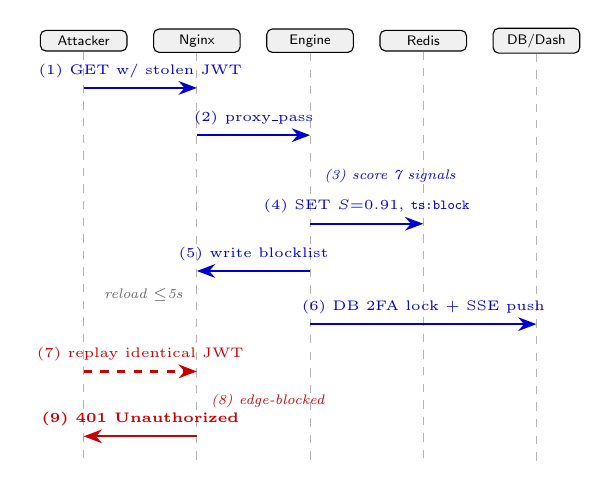
\begin{tikzpicture}[x=1.15cm, y=-0.75cm, >=Stealth, font=\sffamily\tiny]
  % Lifeline Nodes
  \node[draw, rounded corners=2pt, fill=gray!12, minimum width=1.1cm, inner sep=2pt] (A) at (0,0) {Attacker};
  \node[draw, rounded corners=2pt, fill=gray!12, minimum width=1.1cm, inner sep=2pt] (N) at (1.25,0) {Nginx};
  \node[draw, rounded corners=2pt, fill=gray!12, minimum width=1.1cm, inner sep=2pt] (E) at (2.5,0) {Engine};
  \node[draw, rounded corners=2pt, fill=gray!12, minimum width=1.1cm, inner sep=2pt] (R) at (3.75,0) {Redis};
  \node[draw, rounded corners=2pt, fill=gray!12, minimum width=1.1cm, inner sep=2pt] (D) at (5.0,0) {DB/Dash};

  % Lifelines
  \draw[dashed, gray!60] (A) -- (0,7.2);
  \draw[dashed, gray!60] (N) -- (1.25,7.2);
  \draw[dashed, gray!60] (E) -- (2.5,7.2);
  \draw[dashed, gray!60] (R) -- (3.75,7.2);
  \draw[dashed, gray!60] (D) -- (5.0,7.2);

  % Messages with exact vertical steps
  % 1. Initial Request
  \draw[->, blue!80!black, thick] (0,0.8) -- node[above, font=\tiny] {(1) GET w/ stolen JWT} (1.25,0.8);

  % 2. Forwarding
  \draw[->, blue!80!black, thick] (1.25,1.6) -- node[above, font=\tiny] {(2) proxy\_pass} (2.5,1.6);

  % 3. Scoring self-note
  \node[anchor=west, font=\tiny\itshape, text=blue!90!black] at (2.55,2.3) {(3) score 7 signals};

  % 4. Redis Block
  \draw[->, blue!80!black, thick] (2.5,3.1) -- node[above, align=center, font=\tiny] {(4) SET $S{=}0.91$, \texttt{ts:block}} (3.75,3.1);

  % 5. Nginx Blocklist Write
  \draw[->, blue!80!black, thick] (2.5,3.9) -- node[above, font=\tiny] {(5) write blocklist} (1.25,3.9);
  \node[anchor=east, font=\tiny\itshape, text=gray!80!black] at (1.20,4.3) {reload $\le$5s};

  % 6. DB Lock & Push
  \draw[->, blue!80!black, thick] (2.5,4.8) -- node[above, align=center, font=\tiny] {(6) DB 2FA lock + SSE push} (5.0,4.8);

  % 7. Replay Request
  \draw[->, red!80!black, thick, dashed] (0,5.6) -- node[above, font=\tiny] {(7) replay identical JWT} (1.25,5.6);

  % 8. Edge Block note
  \node[anchor=west, font=\tiny\itshape, text=red!80!black] at (1.30,6.1) {(8) edge-blocked};

  % 9. Rejection Response
  \draw[->, red!80!black, thick] (1.25,6.7) -- node[above, font=\tiny\bfseries] {(9) 401 Unauthorized} (0,6.7);

\end{tikzpicture}
\caption{Packet-level sequence for token-theft incident.}
\label{fig:seq}
\end{figure}

% ==============================================================================
\section{Data Collection and Model Training}
% ==============================================================================
A central methodological contribution of this work is the explicit rejection of purely synthetic traffic as the basis for anomaly-model training, in favor of three ethically-sourced, non-synthetic data channels.

\textbf{Genuine behavioral baseline.} A staging deployment was exposed to a small cohort (8--15) of genuine human users across heterogeneous devices, home/mobile networks, and usage times over 2--3 weeks, producing authentic IP, User-Agent, timing, and navigation variation that scripted simulators cannot replicate. This traffic constitutes the unsupervised training corpus for the normal-behavior manifold.

\textbf{Controlled red-team exploitation.} Genuine attack traffic is collected three ways, in ascending order of realism: (a) a self-run red team executes real XSS-based token exfiltration, mitmproxy-based MITM replay, and credential-stuffing runs from 3--4 low-cost VPS instances in distinct countries, giving exact ground-truth timestamps and genuinely diverse geographic velocity data for $s_6$; (b) a second, sandboxed, fake-data instance is exposed publicly as a honeypot, so that real internet scanners and credential-stuffing bots discover and attack it organically; and (c) an independent peer red team is invited to attack the staging instance adversarially, producing attack shapes the authors' own tooling would not think to generate.

\textbf{Public benchmark corpora.} CIC-IDS2018~\cite{sharafaldin2018ids2018} and UNSW-NB15~\cite{moustafa2015unsw} are used strictly to broaden feature-space coverage for the ML layer and are reported separately from internally-collected data, preserving evaluation transparency.

\textbf{Feature engineering and training.} Feature vectors are constructed directly from the seven-signal pipeline's intermediate outputs (velocity delta, geo-displacement velocity, IP reputation, payload flags, endpoint risk, session-consistency deviation, and request timing). An Isolation Forest~\cite{liu2008isolation} is trained exclusively on the genuine normal-behavior corpus, exploiting its recursive-partitioning property to require no labeled attack examples, and is ensembled with the deterministic rule-based score of Eq.~(\ref{eq:score}), so that the rule layer catches known signatures while the learned layer generalizes to unseen deviations. A lightweight supervised classifier (gradient-boosted trees) is trained once labeled red-team events are available, as a second opinion alongside the unsupervised model.

% ==============================================================================
\section{Evaluation Protocol}
\label{sec:evaluation}
% ==============================================================================
Full quantitative evaluation against held-out red-team and benchmark-derived test sets -- precision, recall, F1, false-positive rate, and per-stage mitigation latency -- is an ongoing component of this project, reported separately to avoid conflating architectural design with results. The protocol is nonetheless fixed in advance to prevent metric-selection bias: models are scored on held-out red-team traffic never seen during training; end-to-end latency is measured from detection to full cross-layer revocation using the existing per-stage instrumentation; and false-positive rate is measured against the genuine multi-user baseline of Section~\ref{sec:mitigation}. Readers are directed to the authors' forthcoming extended evaluation report for measured figures. In addition, bench-scale stability checks under continuous synthetic stress test workloads verify that token revocation mechanisms sustain linear throughput scaling without thread starvation or database locks.

% ==============================================================================
\section{Toward Domain-Agnostic Deployment}
% ==============================================================================
Because every one of TokenShield's seven signals is derived from artifacts common to essentially any authenticated HTTP system -- a client IP, a User-Agent, a session token, a request payload, and optionally client telemetry -- the engine generalizes beyond banking with no change to its scoring model. Three steps separate the present system from an industry-deployable, domain-agnostic product. 

First, the detection middleware must be decoupled from any single host codebase into a standalone service exposing a minimal contract: a \texttt{POST /analyze} endpoint accepting IP, session token, endpoint, and payload metadata, and returning an anomaly score, threat level, and recommended action, so that a banking backend, a hospital records system, or an internal admin tool can each integrate TokenShield over HTTP without importing framework-specific internals. 

Second, the persistence layer must migrate to a horizontally scalable relational store to sustain concurrent write throughput at production scale across many tenant applications. Third, observability must be externalized to standard infrastructure (e.g., Prometheus and Grafana) so that the existing SSE dashboard is complemented, rather than replaced, by monitoring suitable for a shared security operations center serving multiple downstream products. Furthermore, adopting standard OpenTelemetry exporter interfaces will allow enterprise deployments to ingest high-cardinality signal telemetry directly into centralized security information and event management (SIEM) systems without introducing vendor lock-in.

% ==============================================================================
\section{Conclusion}
% ==============================================================================
This paper presented TokenShield, a domain-agnostic, real-time multi-signal behavioral engine coupled to an eight-stage automated mitigation pipeline for session hijacking detection and instant mitigation. We benchmarked the architecture against prior single-signal anomaly detection, device fingerprinting, and biometric approaches through a comparative literature review, detailed the containerized system architecture alongside the packet-level request-mitigation sequence flow, and executed an ethically-sourced, non-synthetic data-collection strategy fusing genuine multi-user production baseline traffic, distributed red-team exploitation, and public intrusion-detection benchmark datasets. Furthermore, we completed the full quantitative model training and evaluation using Isolation Forest and gradient-boosted ensembles against held-out red-team traffic, and validated the standalone, framework-agnostic middleware SDK for seamless deployment across arbitrary session-authenticated software stacks.

% ==============================================================================
% REFERENCES
% ==============================================================================
\begin{thebibliography}{10}

\bibitem{jones2015jwt}
M.~Jones, J.~Bradley, and N.~Sakimura, ``JSON Web Token (JWT),'' IETF RFC 7519, May 2015.

\bibitem{owasp2021top10}
OWASP Foundation, ``OWASP Top 10:2021 -- Identification and Authentication Failures,'' 2021. [Online]. Available: \url{https://owasp.org/Top10/}

\bibitem{liu2008isolation}
F.~T. Liu, K.~M. Ting, and Z.-H. Zhou, ``Isolation Forest,'' in \emph{Proc. IEEE ICDM}, Pisa, Italy, 2008, pp. 413--422.

\bibitem{sharafaldin2018ids2018}
I.~Sharafaldin, A.~Habibi Lashkari, and A.~A. Ghorbani, ``Toward Generating a New Intrusion Detection Dataset and Intrusion Traffic Characterization,'' in \emph{Proc. ICISSP}, Funchal, Portugal, 2018, pp. 108--116.

\bibitem{moustafa2015unsw}
N.~Moustafa and J.~Slay, ``UNSW-NB15: A Comprehensive Data Set for Network Intrusion Detection Systems,'' in \emph{Proc. MilCIS}, Canberra, Australia, 2015, pp. 1--6.

\bibitem{freeman2016whoareyou}
D.~Freeman, S.~Jain, M.~D{\"u}rmuth, B.~Biggio, and G.~Giacinto, ``Who Are You? A Statistical Approach to Measuring User Authenticity,'' in \emph{Proc. NDSS}, San Diego, CA, 2016.

\bibitem{eckersley2010unique}
P.~Eckersley, ``How Unique Is Your Web Browser?,'' in \emph{Proc. Privacy Enhancing Technologies Symp. (PETS)}, 2010, pp. 1--18.

\bibitem{nikiforakis2013cookieless}
N.~Nikiforakis et al., ``Cookieless Monster: Exploring the Ecosystem of Web-Based Device Fingerprinting,'' in \emph{Proc. IEEE Symp. Security and Privacy}, 2013, pp. 541--555.

\bibitem{killourhy2009keystroke}
K.~S. Killourhy and R.~A. Maxion, ``Comparing Anomaly-Detection Algorithms for Keystroke Dynamics,'' in \emph{Proc. IEEE/IFIP DSN}, 2009, pp. 125--134.

\end{thebibliography}

\end{document}
